\chapter{Introduzione}
Negli ultimi anni, la mole di dati prodotta da aziende e privati sta crescendo esponenzialmente, tanto che, entro il 2022, si stima che in media si avranno 50 dispositivi connessi a Internet per abitazione \cite{iotedge}. Ovviamente questi dati necessitano di essere processati e conservati, oltre che condivisi tra più dispositivi all'occorrenza. A tal fine, la modalità che si è adottata maggiormente negli ultimi anni è quella del Cloud Computing: i dati non vengono processati in locale per mancanza di risorse, ma inviati a specifici data center online in grado di elaborarli e processarli, oltre che conservarli. Tale approccio introduce però alcune criticità:
\begin{itemize}
	\item \textbf{Latenza}: in molti ambiti è richiesta un'elaborazione dei dati in tempo reale, si pensi per esempio ad un'eventuale applicazione che permetta a un veicolo autonomo di riconoscere i pedoni. In questo specifico caso è richiesta una bassissima latenza dato l'enorme rischio in gioco. Tuttavia, proprio l'invio dei dati al Cloud, la successiva elaborazione degli stessi e, infine, l'invio di un feedback al dispositivo in uso, introducono ritardi non trascurabili, pertanto in questi specifici casi il Cloud Computing risulta non essere l'approccio migliore.
	\item \textbf{Scalabilità}: l'invio dei dati al Cloud è problematico in tal senso, dato soprattutto il numero in crescita esponenziale di dispositivi connessi. Inoltre, l'invio di tutti i dati al Cloud è inefficiente in termini di consumo di risorse, in particolare se non tutti i dati sono necessari al Deep Learning.
	\item \textbf{Privacy}: l'invio di dati sensibili a server online aumenta i rischi di furto di tali informazioni, oltre al fatto che l'utente spesso e volentieri non è a conoscenza di come questi dati verranno trattati né tantomeno di dove saranno conservati.
\end{itemize}
Una possibile soluzione a queste tre criticità, proprie del Cloud Computing, è l'Edge Computing (si veda figura \ref{edge}). 
\begin{figure}[H]
	\centering
	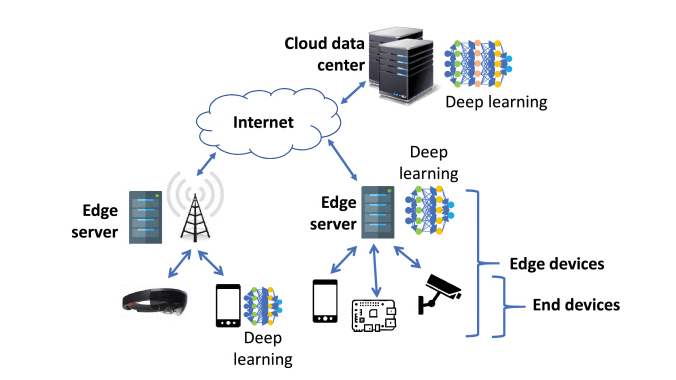
\includegraphics[width=\linewidth, height= 0.3 \textheight]{pics/edgecomputing.jpeg}
	\caption{Struttura dell'Edge Computing}
	\label{edge}
\end{figure}
Tale approccio prevede una rete di micro data center posti nelle vicinanze dei dispositivi che rilevano i dati da elaborare. Proprio questa vicinanza alle sorgenti dei dati permette di ridurre drasticamente la latenza (si veda figura \ref{edgevs}). Inoltre, al fine di incrementare le prestazioni in termini di scalabilità, è prevista una struttura gerarchica dei dispositivi connessi, oltre al fatto che non è necessario apportare modifiche o espansioni ai data center in Cloud siccome i dati vengono elaborati in locale. Per quanto riguarda infine i vincoli di privacy, l'Edge Computing prevede l'elaborazione dei dati alla sorgente, solitamente grazie a un server locale, perciò i dati non vengono trasmessi sulla rete globale, riducendo dunque i rischi che ne deriverebbero.
\begin{figure}[H]
	\centering
	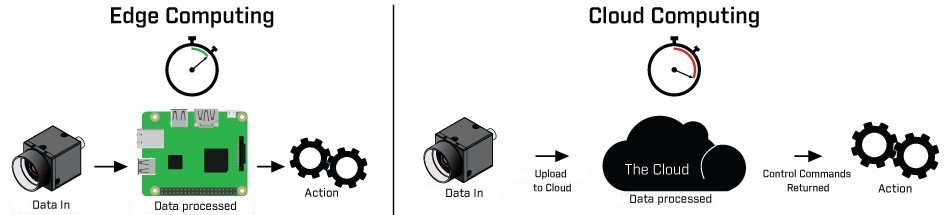
\includegraphics[width=\linewidth, height= 0.15 \textheight]{pics/edgevscloud.jpeg}
	\caption{Confronto tra Edge e Cloud Computing}
	\label{edgevs}
\end{figure}
L'approccio Edge Computing presenta però alcune criticità.\\
Uno degli aspetti più importanti da considerare è l'elevata quantità di risorse richiesta da determinati algoritmi (come ad esempio quelli di Machine Learning o di elaborazione delle immagini), in contrapposizione con l'utilizzo di nodi locali dotati di ridotta potenza di calcolo rispetto ai server centralizzati.\\
Un secondo problema è la coordinazione tra i dispositivi Edge e il Cloud, considerando che per ognuno di essi si avranno verosimilmente differenti capacità di calcolo e tipologie di connessione alla rete.\\
In ultimo, dal lato privacy, anche se le potenziali minacce sono ridotte rispetto a una soluzione unicamente basata sul Cloud Computing, la riservatezza rimane comunque un punto delicato poiché i dati necessitano di essere condivisi tra i vari dispositivi e pertanto risulta necessario l'utilizzo della comunicazione in rete, oltre al fatto che il dispositivo perimetrale avrà meno potenza di calcolo da dedicare a complessi algoritmi di criptazione.\\
Con queste premesse nasce l'idea di realizzare Edge Engine: un runtime system generico, slegato dall'hardware, in grado di interpretare codice per dispositivi multipiattaforma, comprese board di sviluppo per microcontrollori. Tale sistema è in grado di elaborare i flussi di dati provenienti dai sensori ad esso collegati grazie all'utilizzo degli script: insiemi di operazioni prestabilite che possono anche essere composte al fine di eseguire calcoli complessi sui dati in ingresso. L'Edge Engine è configurato in modo tale da recuperare dal Cloud gli scripts associati al dispositivo in uso, eseguirli localmente e poi trasmettere nuovamente al Cloud i risultati ottenuti. Per il corretto funzionamento di Edge Engine è dunque necessario un server online che conservi gli scripts e le descrizioni dei vari dispositivi. In questo specifico caso verrà utilizzato Measurify: una piattaforma cloud creata dall'Elios Lab dell'Università di Genova per gestire oggetti smart dell'Internet of Things (IoT).\\
Lo scopo del progetto in esame sarà la realizzazione di Edge Engine per sistemi PC (Windows/Linux/MacOS) e, successivamente, l'impiego di tale motore in un contesto di realtà virtuale, quale un simulatore medico, in modo da illustrare e testare un'ulteriore modalità di impiego del sistema.
\begin{figure}[H]
	\centering
	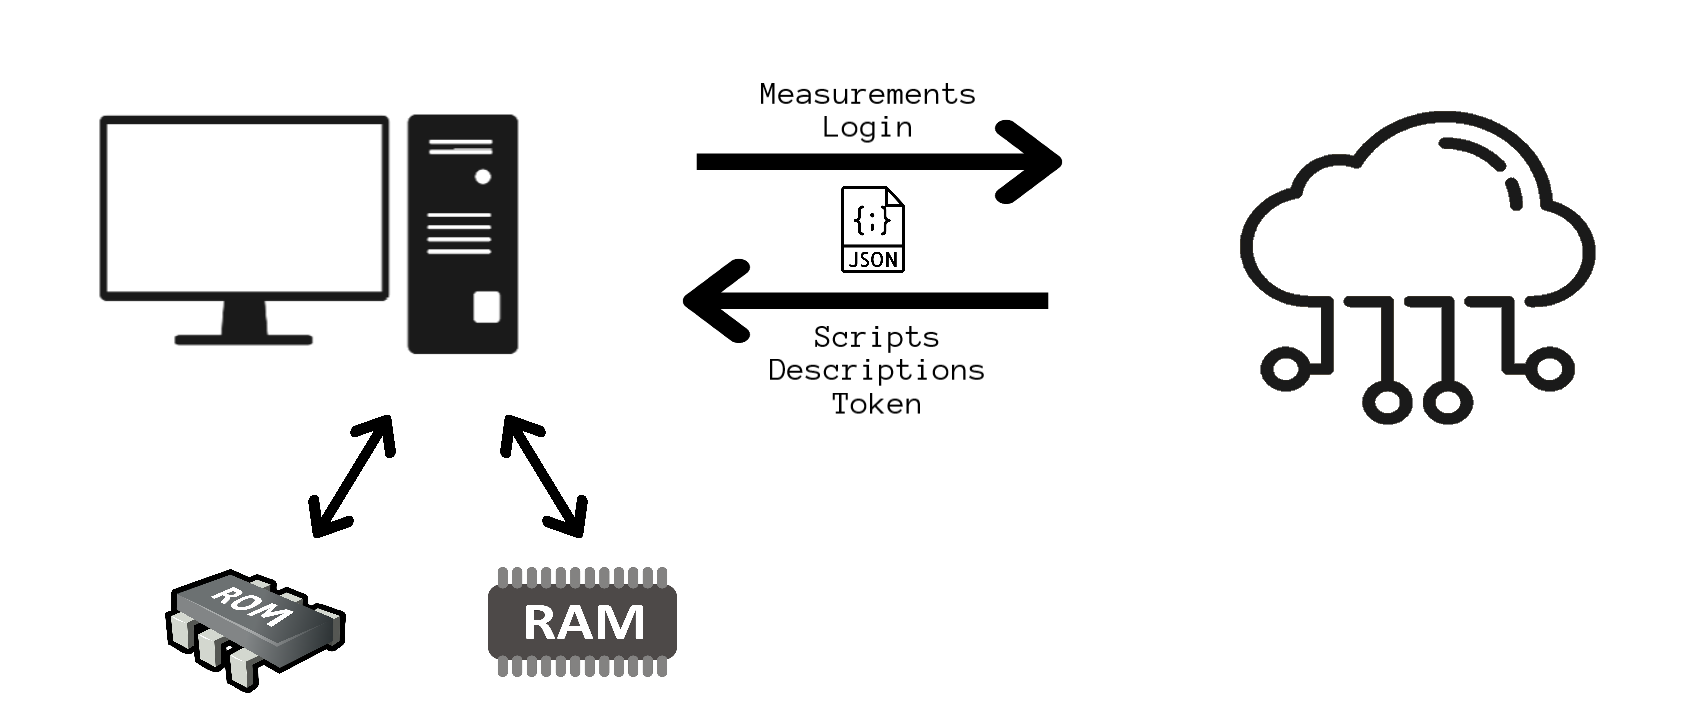
\includegraphics[width=\linewidth, height= 0.25 \textheight]{pics/edgine}
	\caption{Edge Engine per PC}
	\label{edgine}
\end{figure}